\documentclass{article}
\usepackage[utf8]{inputenc}
\usepackage[english]{babel}
\usepackage[font=small,labelfont=bf]{caption}
\usepackage{geometry}
\usepackage{natbib}
\usepackage{pxfonts}
\usepackage{graphicx}
\usepackage{newfloat}
\usepackage{setspace}
%\doublespacing

\newcommand{\argmax}{\mathop{\mathrm{argmax}}\limits}

\title{\textit{Supplementary materials for: } High-level cognition
  during story listening is reflected in high-order dynamic
  correlations in neural activity patterns} \author{Lucy
  L. W. Owen$^1$, Thomas H. Chang$^{1,2}$, and\
  Jeremy R. Manning\textsuperscript{$1, \dagger$}\\
  [0.1in]$^1$Department of Psychological and Brain
  Sciences,\\Dartmouth
  College, Hanover, NH\\
  $^2$Amazon.com, Seattle, WA\\
  \textsuperscript{$\dagger$}Address correspondence to
  jeremy.r.manning@dartmouth.edu}

\bibliographystyle{apa}

\newcommand{\neurosynth}{7}

\begin{document}
\maketitle

\setcounter{equation}{0}
\setcounter{figure}{0}
\setcounter{table}{0}
\setcounter{page}{1}
\setcounter{section}{0}
\makeatletter
\renewcommand{\theequation}{S\arabic{equation}}
\renewcommand{\thefigure}{S\arabic{figure}}
\renewcommand{\bibnumfmt}[1]{[S#1]}
\renewcommand{\citenumfont}[1]{S#1}



\begin{figure}[p!]
\centering
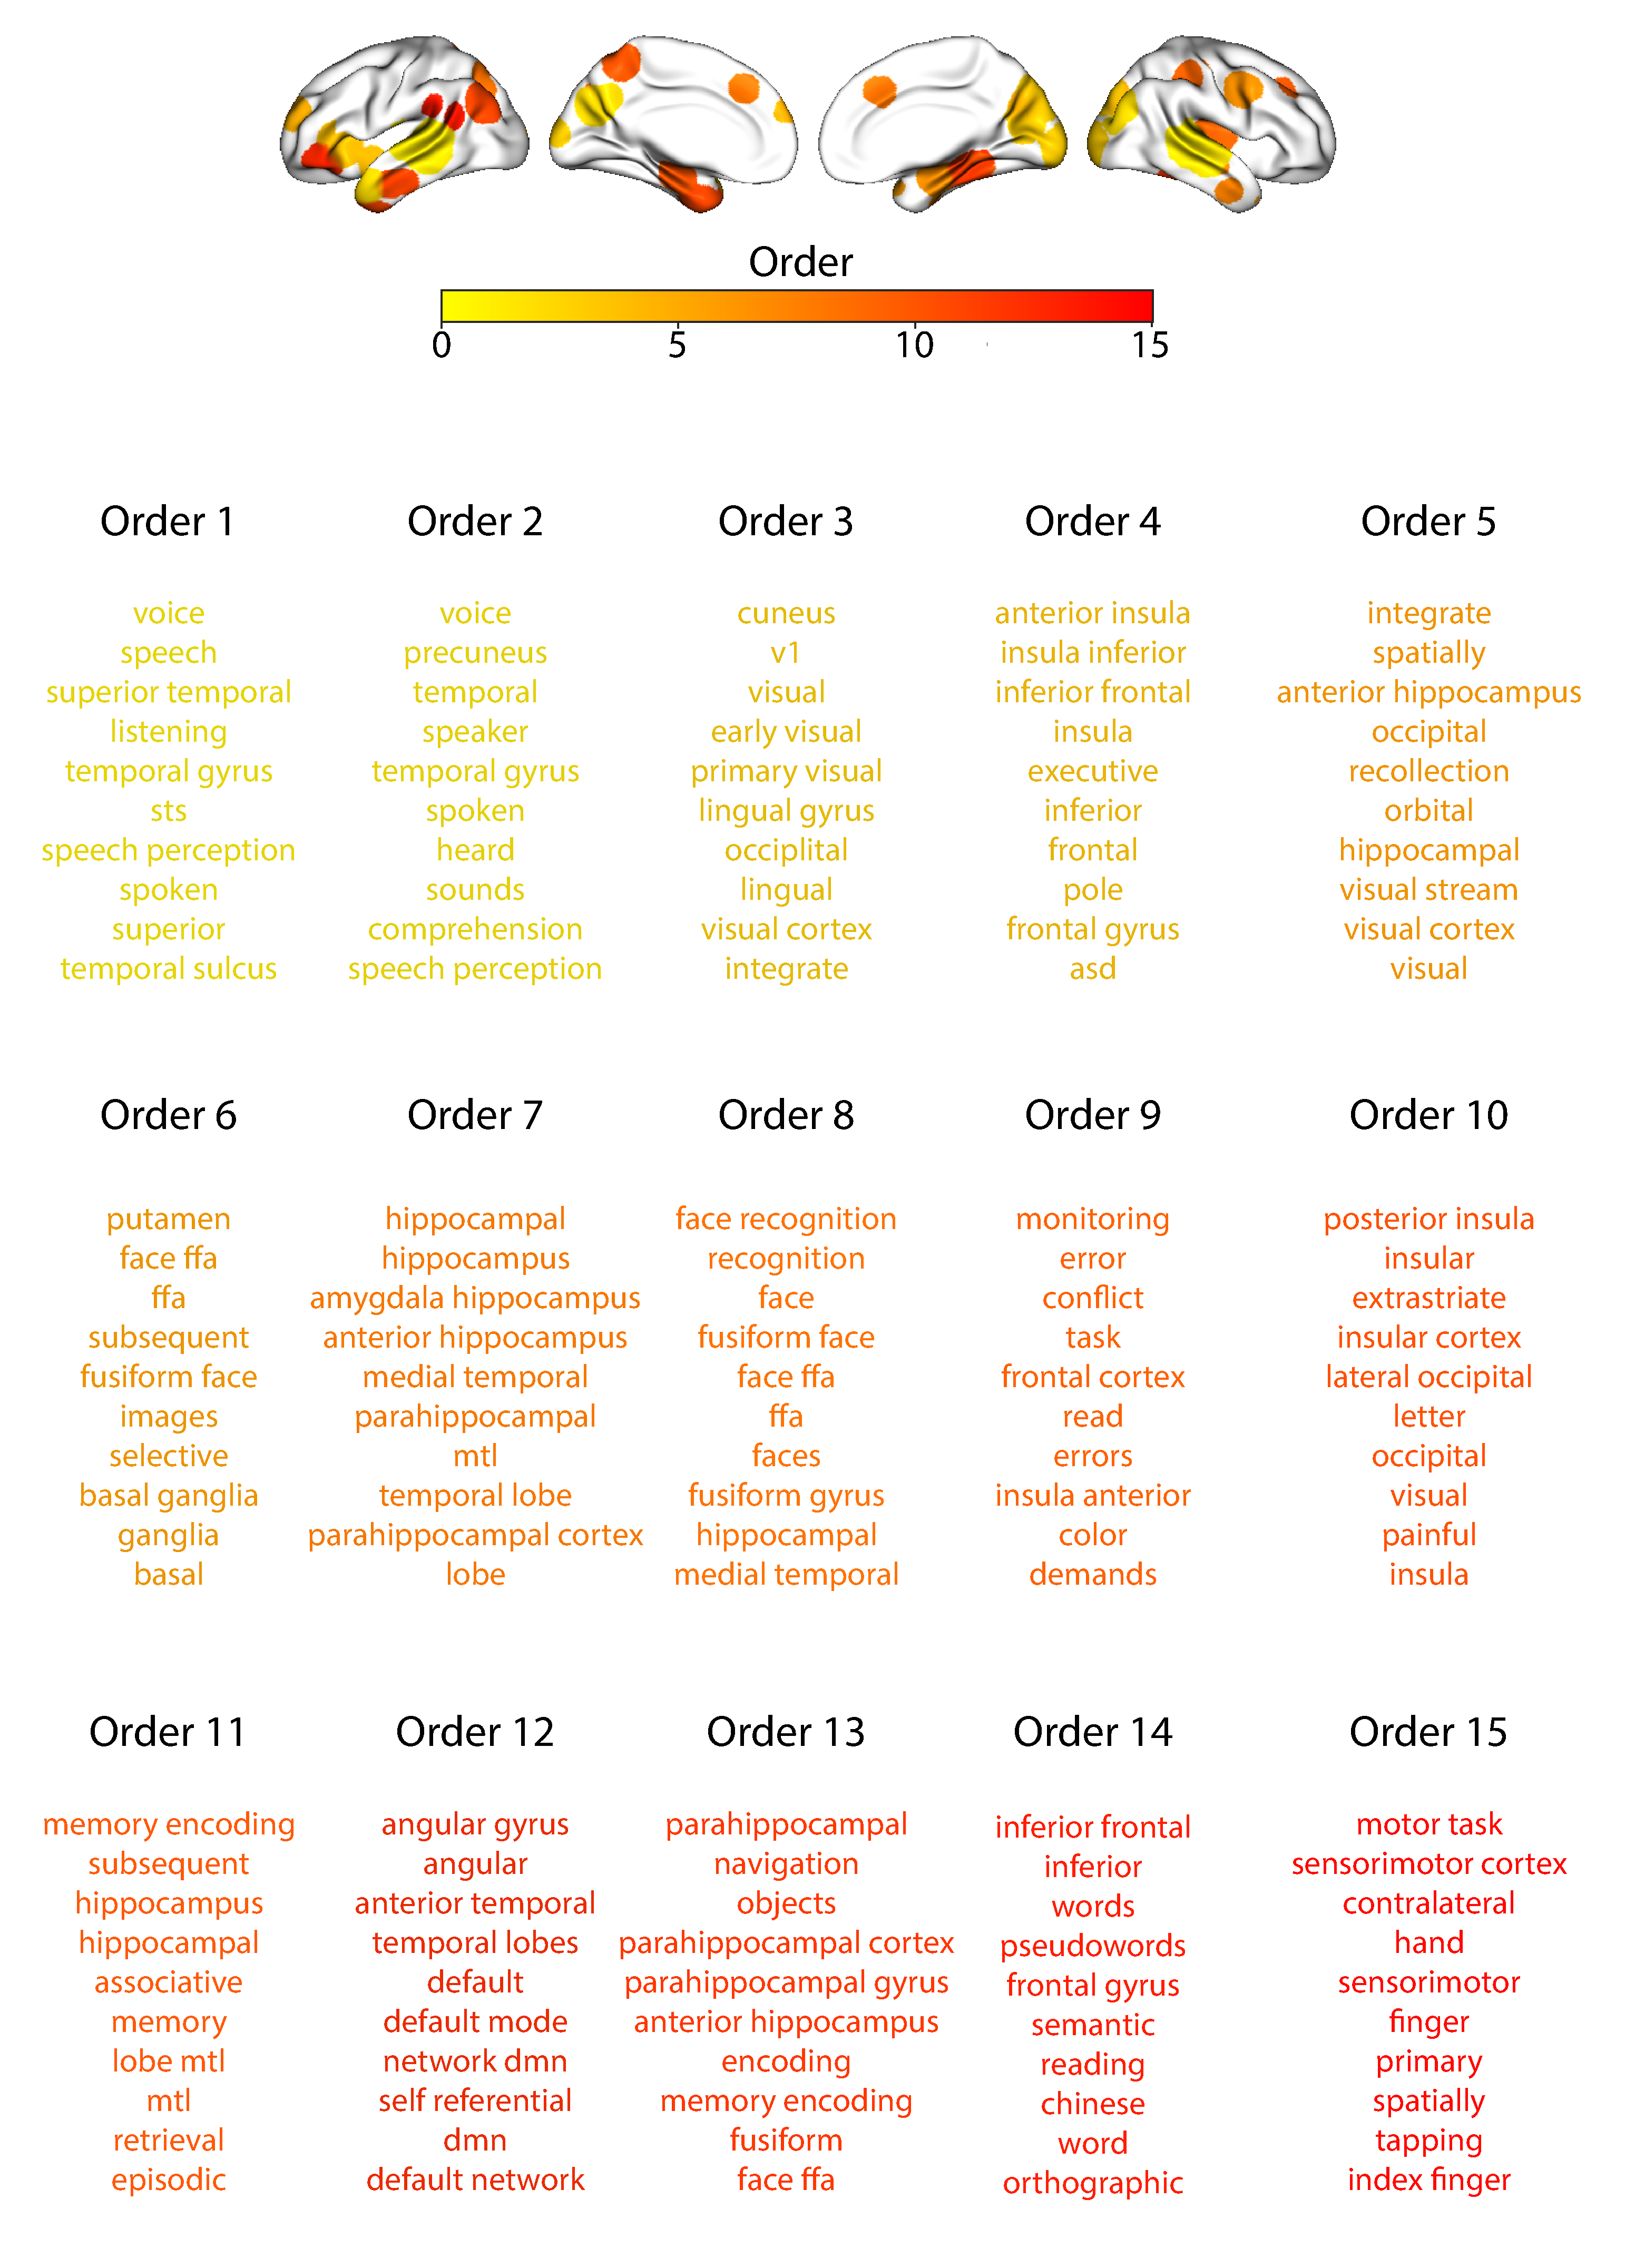
\includegraphics[width=0.75\textwidth]{figs/supp_15_intact}
\caption{\textbf{Top terms associated with the endpoints of the
    strongest correlations for the \textit{intact} experimental
    condition.}  Each color corresponds to one order of inter-subject
functional correlations. The inflated brain plots display the
locations of the endpoints of the 10 strongest (absolute value)
correlations at each order, projected onto the cortical
surface~\citep{CombEtal19}.  The lists of terms display
the top 10 Neurosynth terms~\citep{RubiEtal17} decoded from the
corresponding brain maps for each order.  (Also see Fig.~\neurosynth,
top row, in the main text.)}
\label{fig:intact}
\end{figure}

\begin{figure}[p!]
\centering
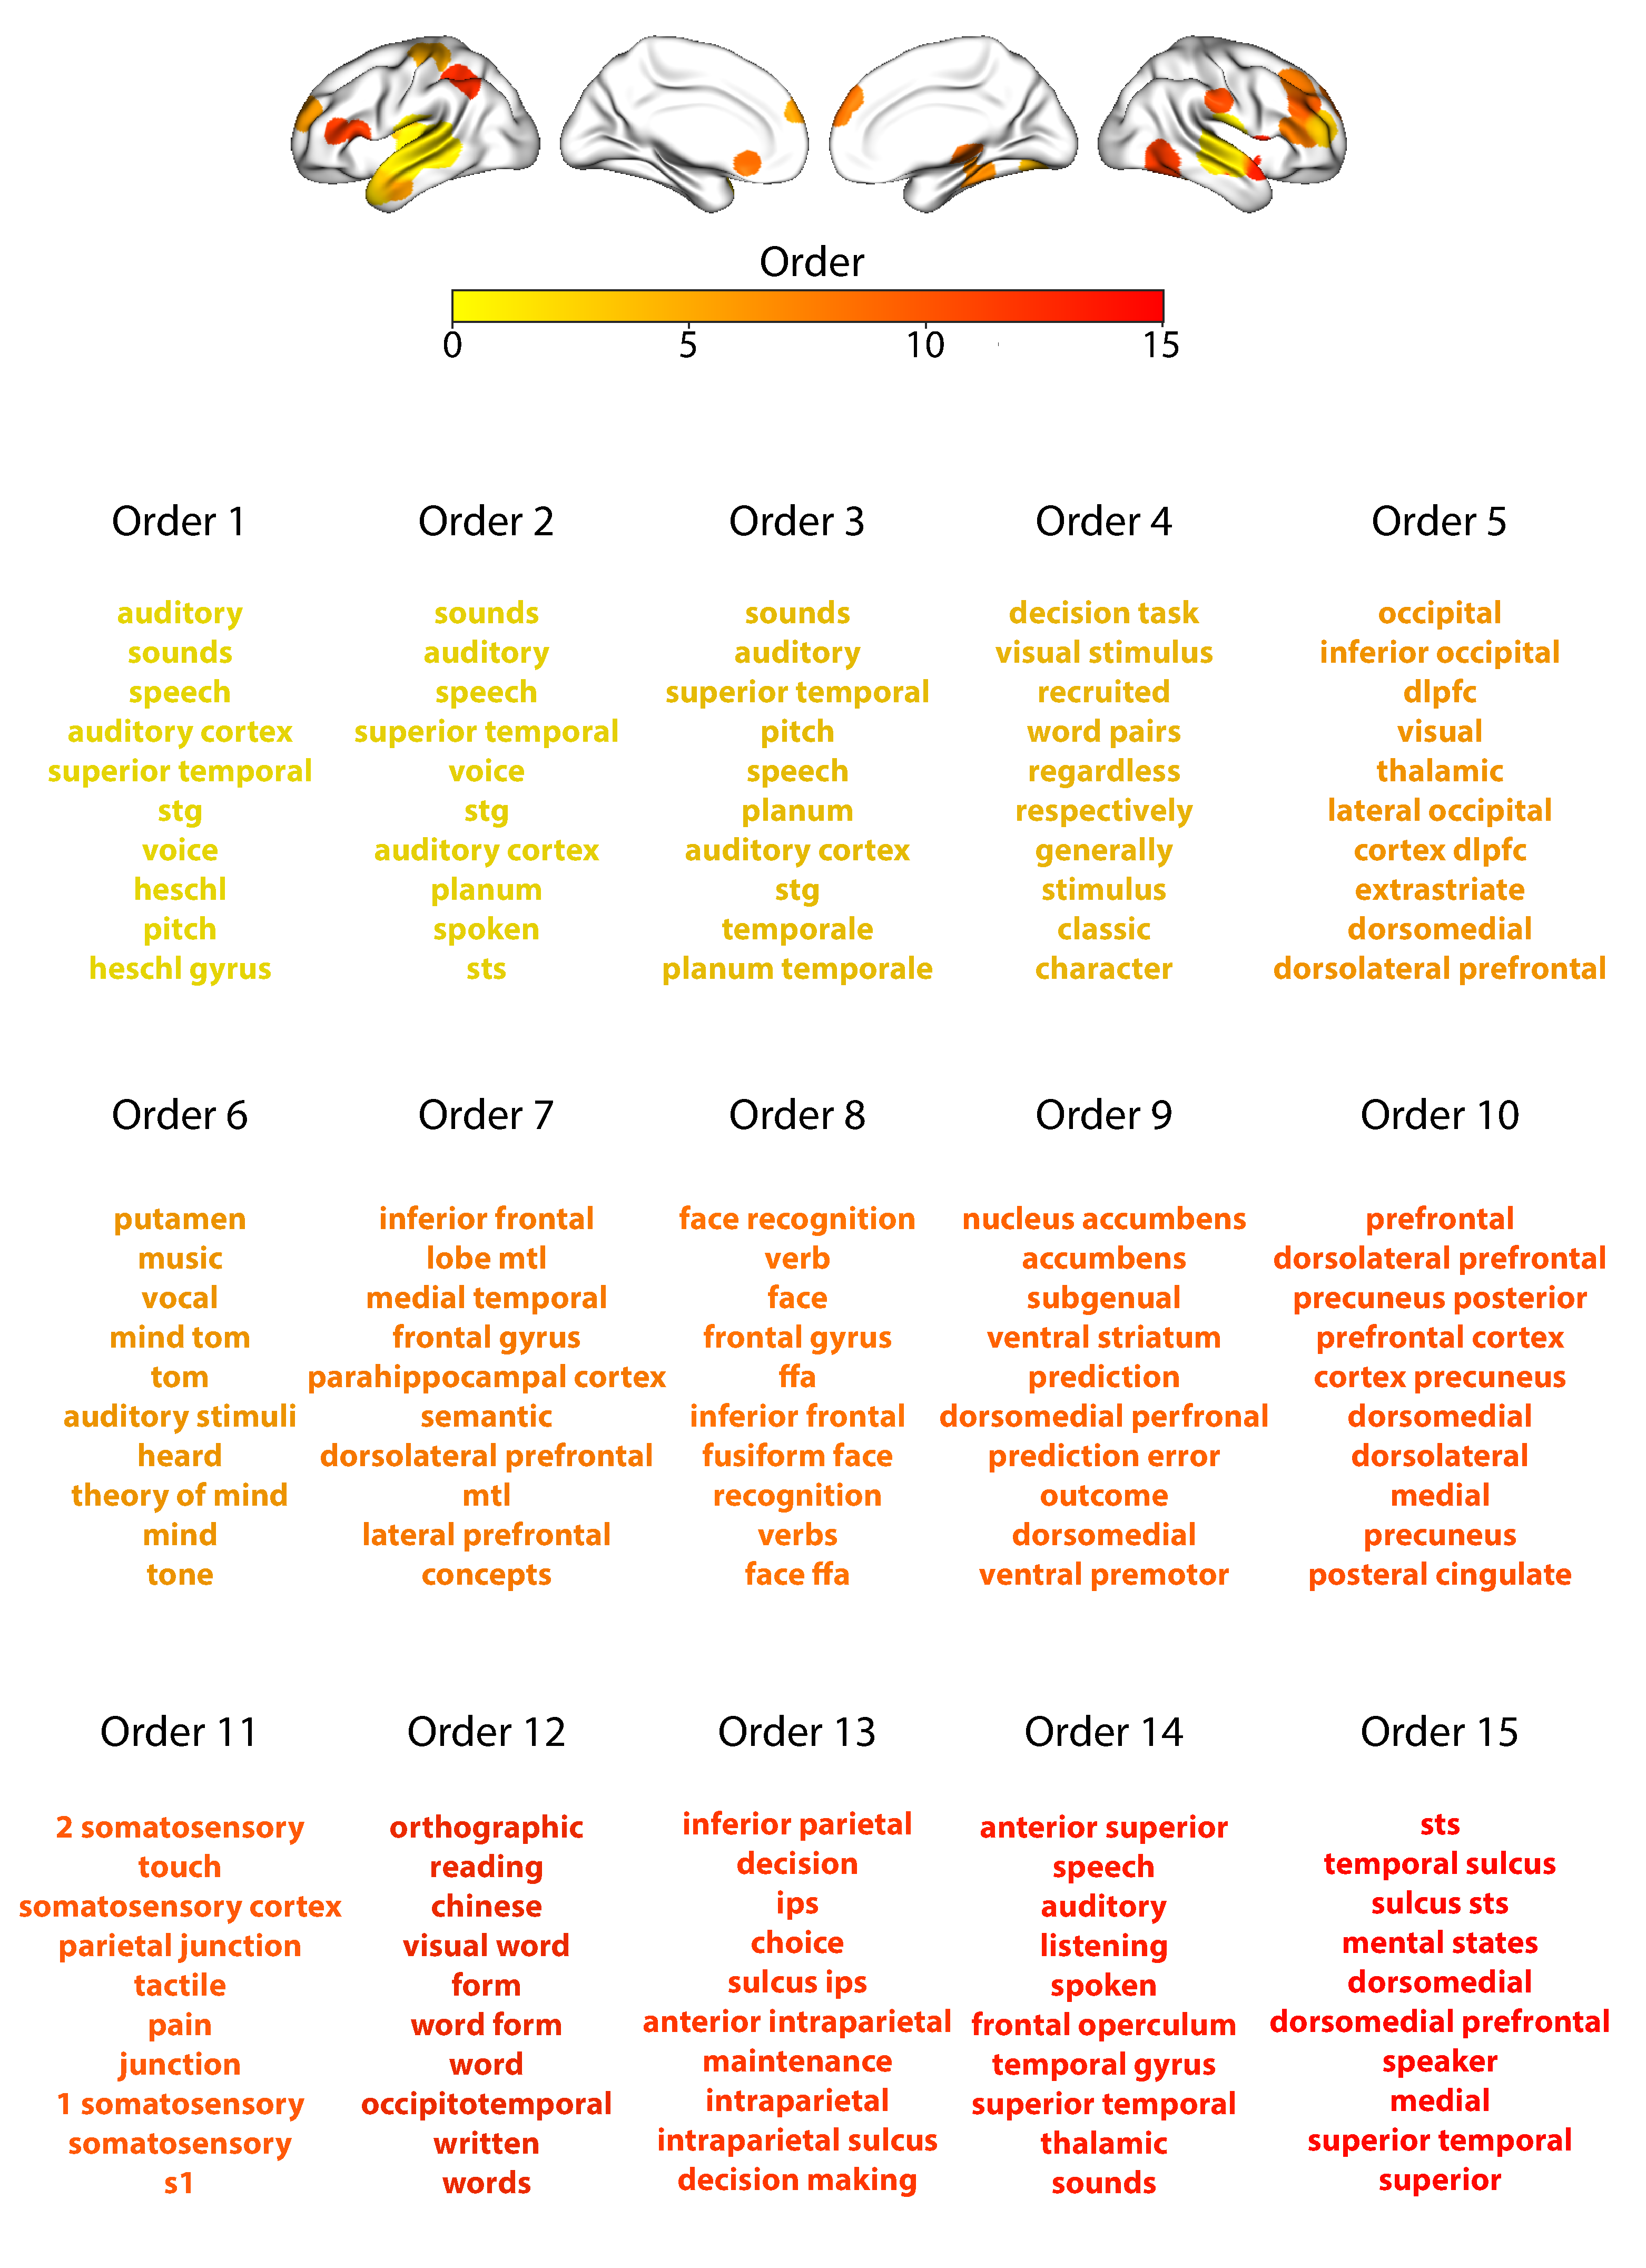
\includegraphics[width=0.75\textwidth]{figs/supp_15_paragraph}
\caption{\textbf{Top terms associated with the endpoints of the
    strongest correlations for the \textit{paragraph} experimental
    condition.}  This figure is in the same format as
  Figure~\ref{fig:intact}, but displays results for the
  paragraph-scrambled story listening condition.  (Also see Fig.~\neurosynth,
second row, in the main text.)}
\label{fig:paragraph}
\end{figure}

\begin{figure}[p!]
\centering
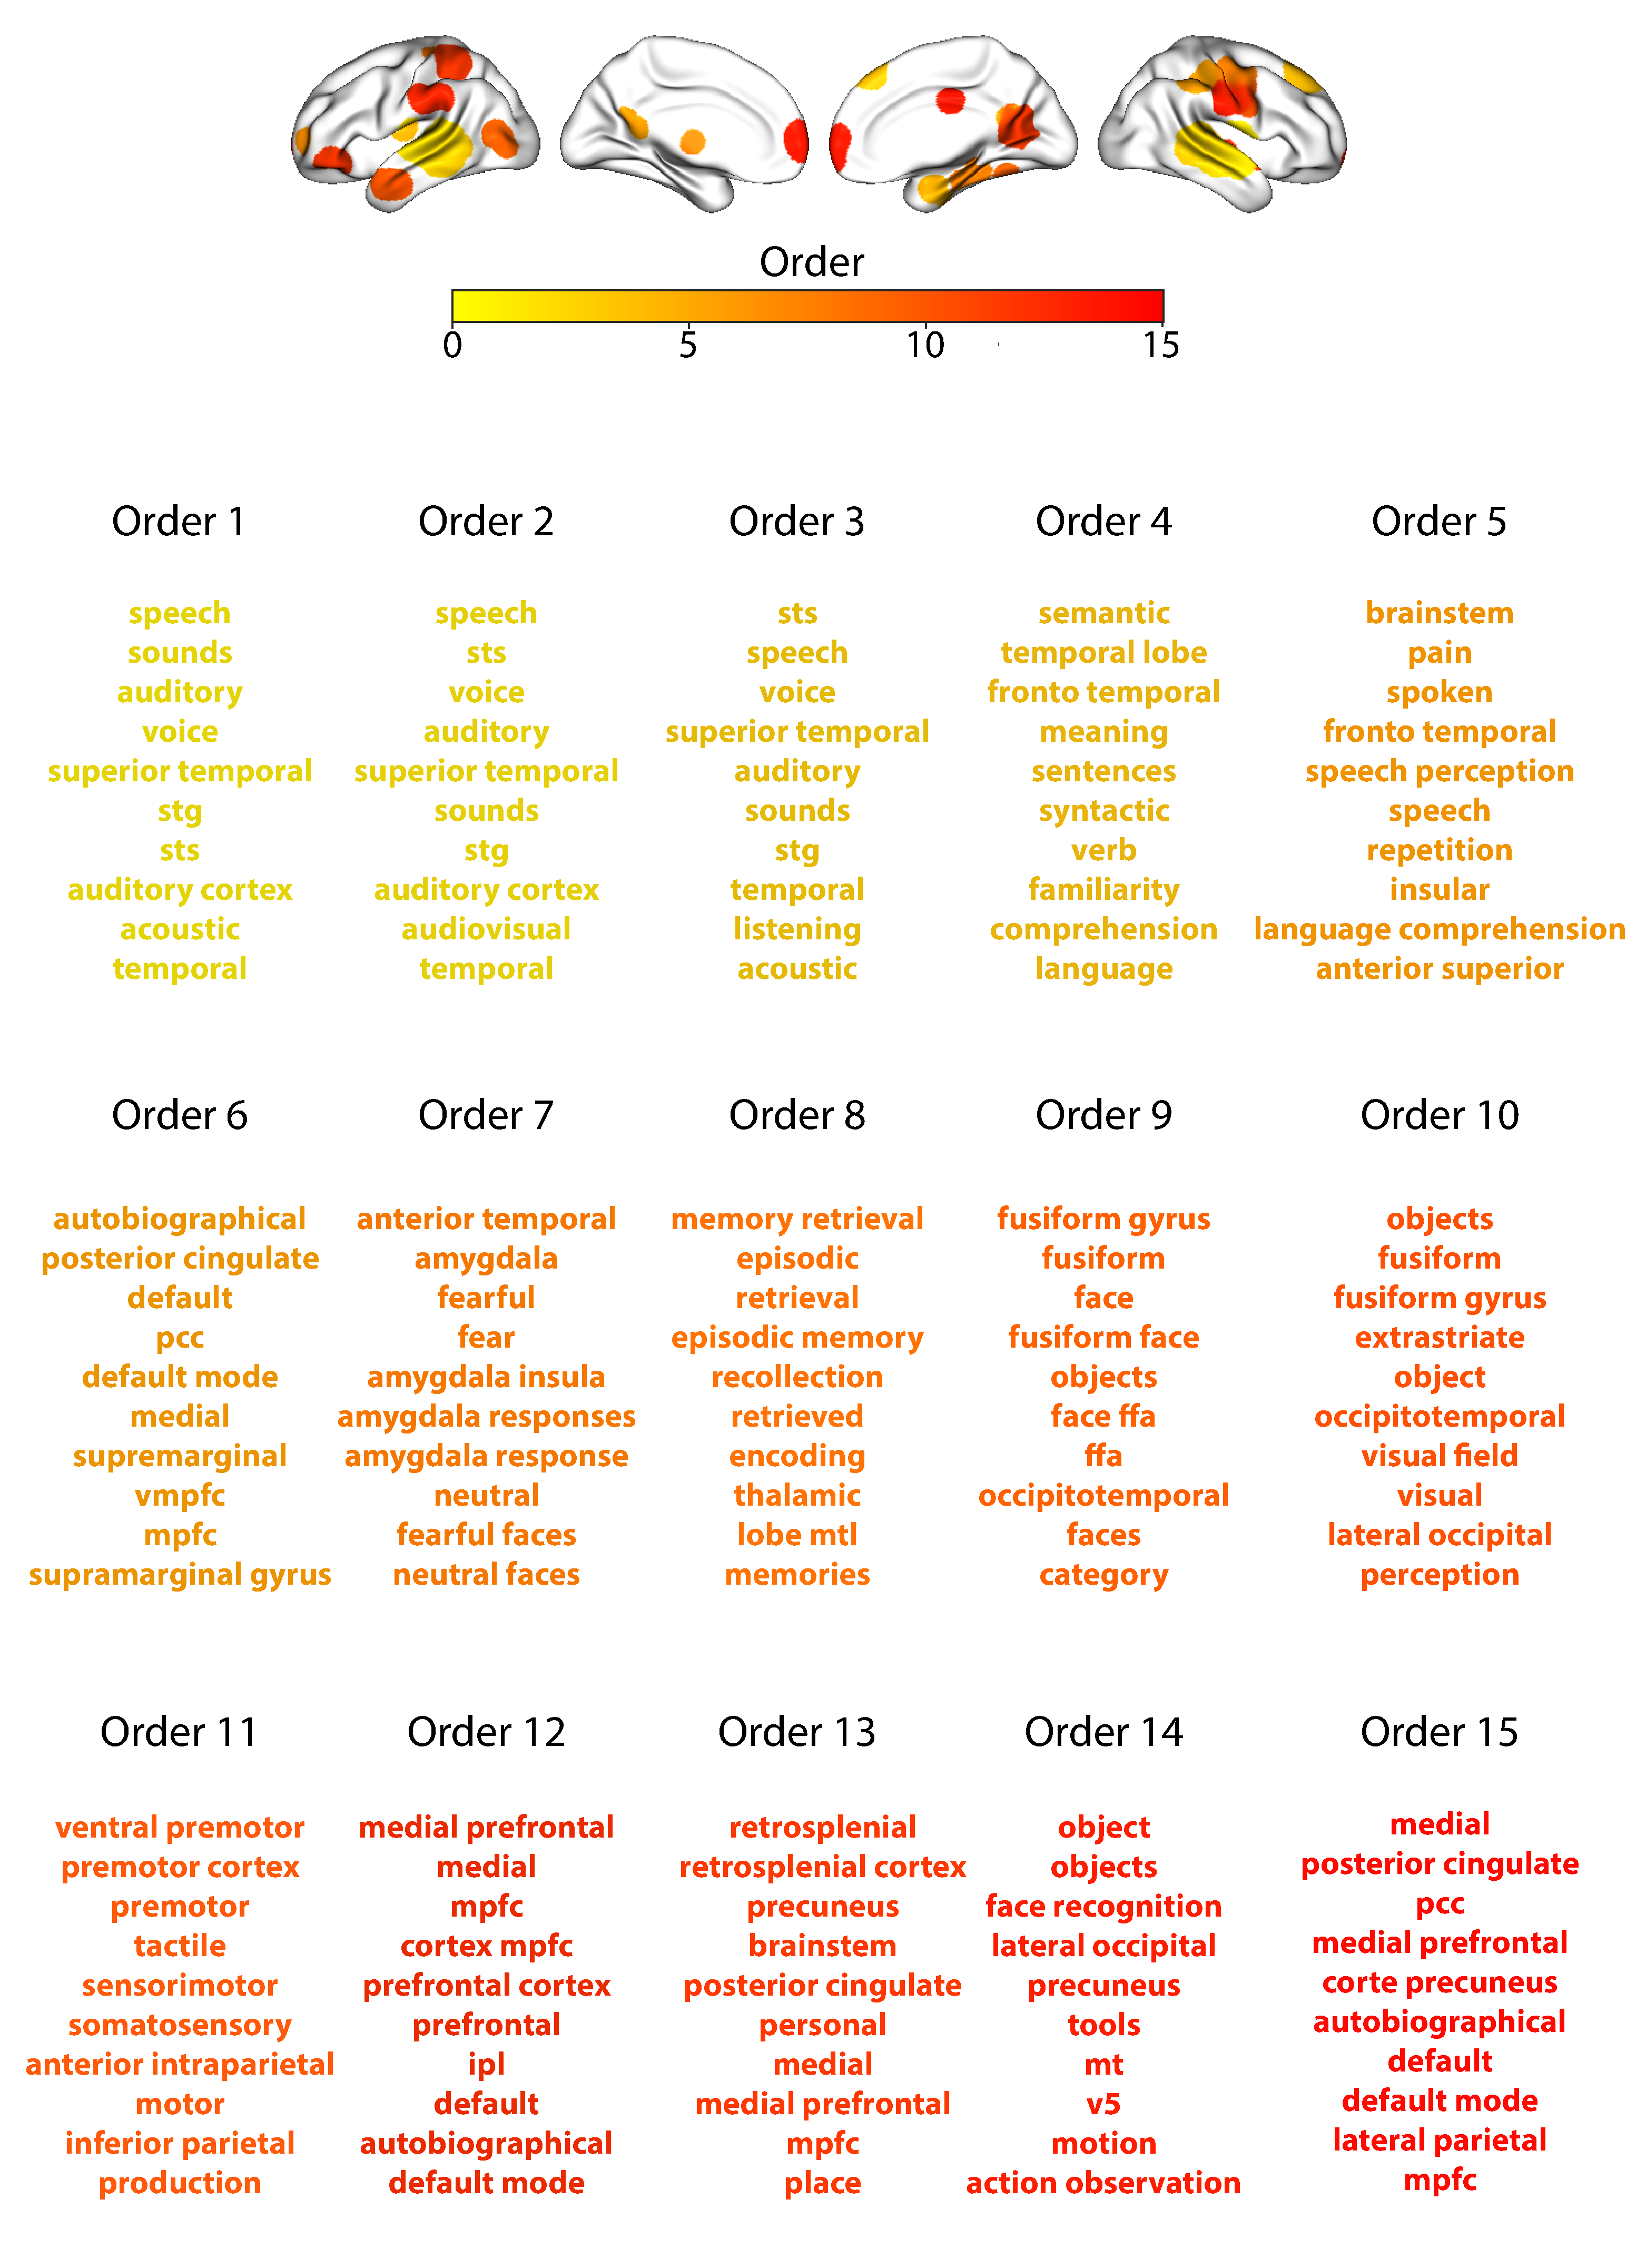
\includegraphics[width=0.75\textwidth]{figs/supp_15_word}
\caption{\textbf{Top terms associated with the endpoints of the
    strongest correlations for the \textit{word} experimental
    condition.}  This figure is in the same format as
  Figure~\ref{fig:intact}, but displays results for the
  word-scrambled story listening condition.  (Also see Fig.~\neurosynth,
third row, in the main text.)}
\label{fig:word}
\end{figure}

\begin{figure}[p!]
\centering
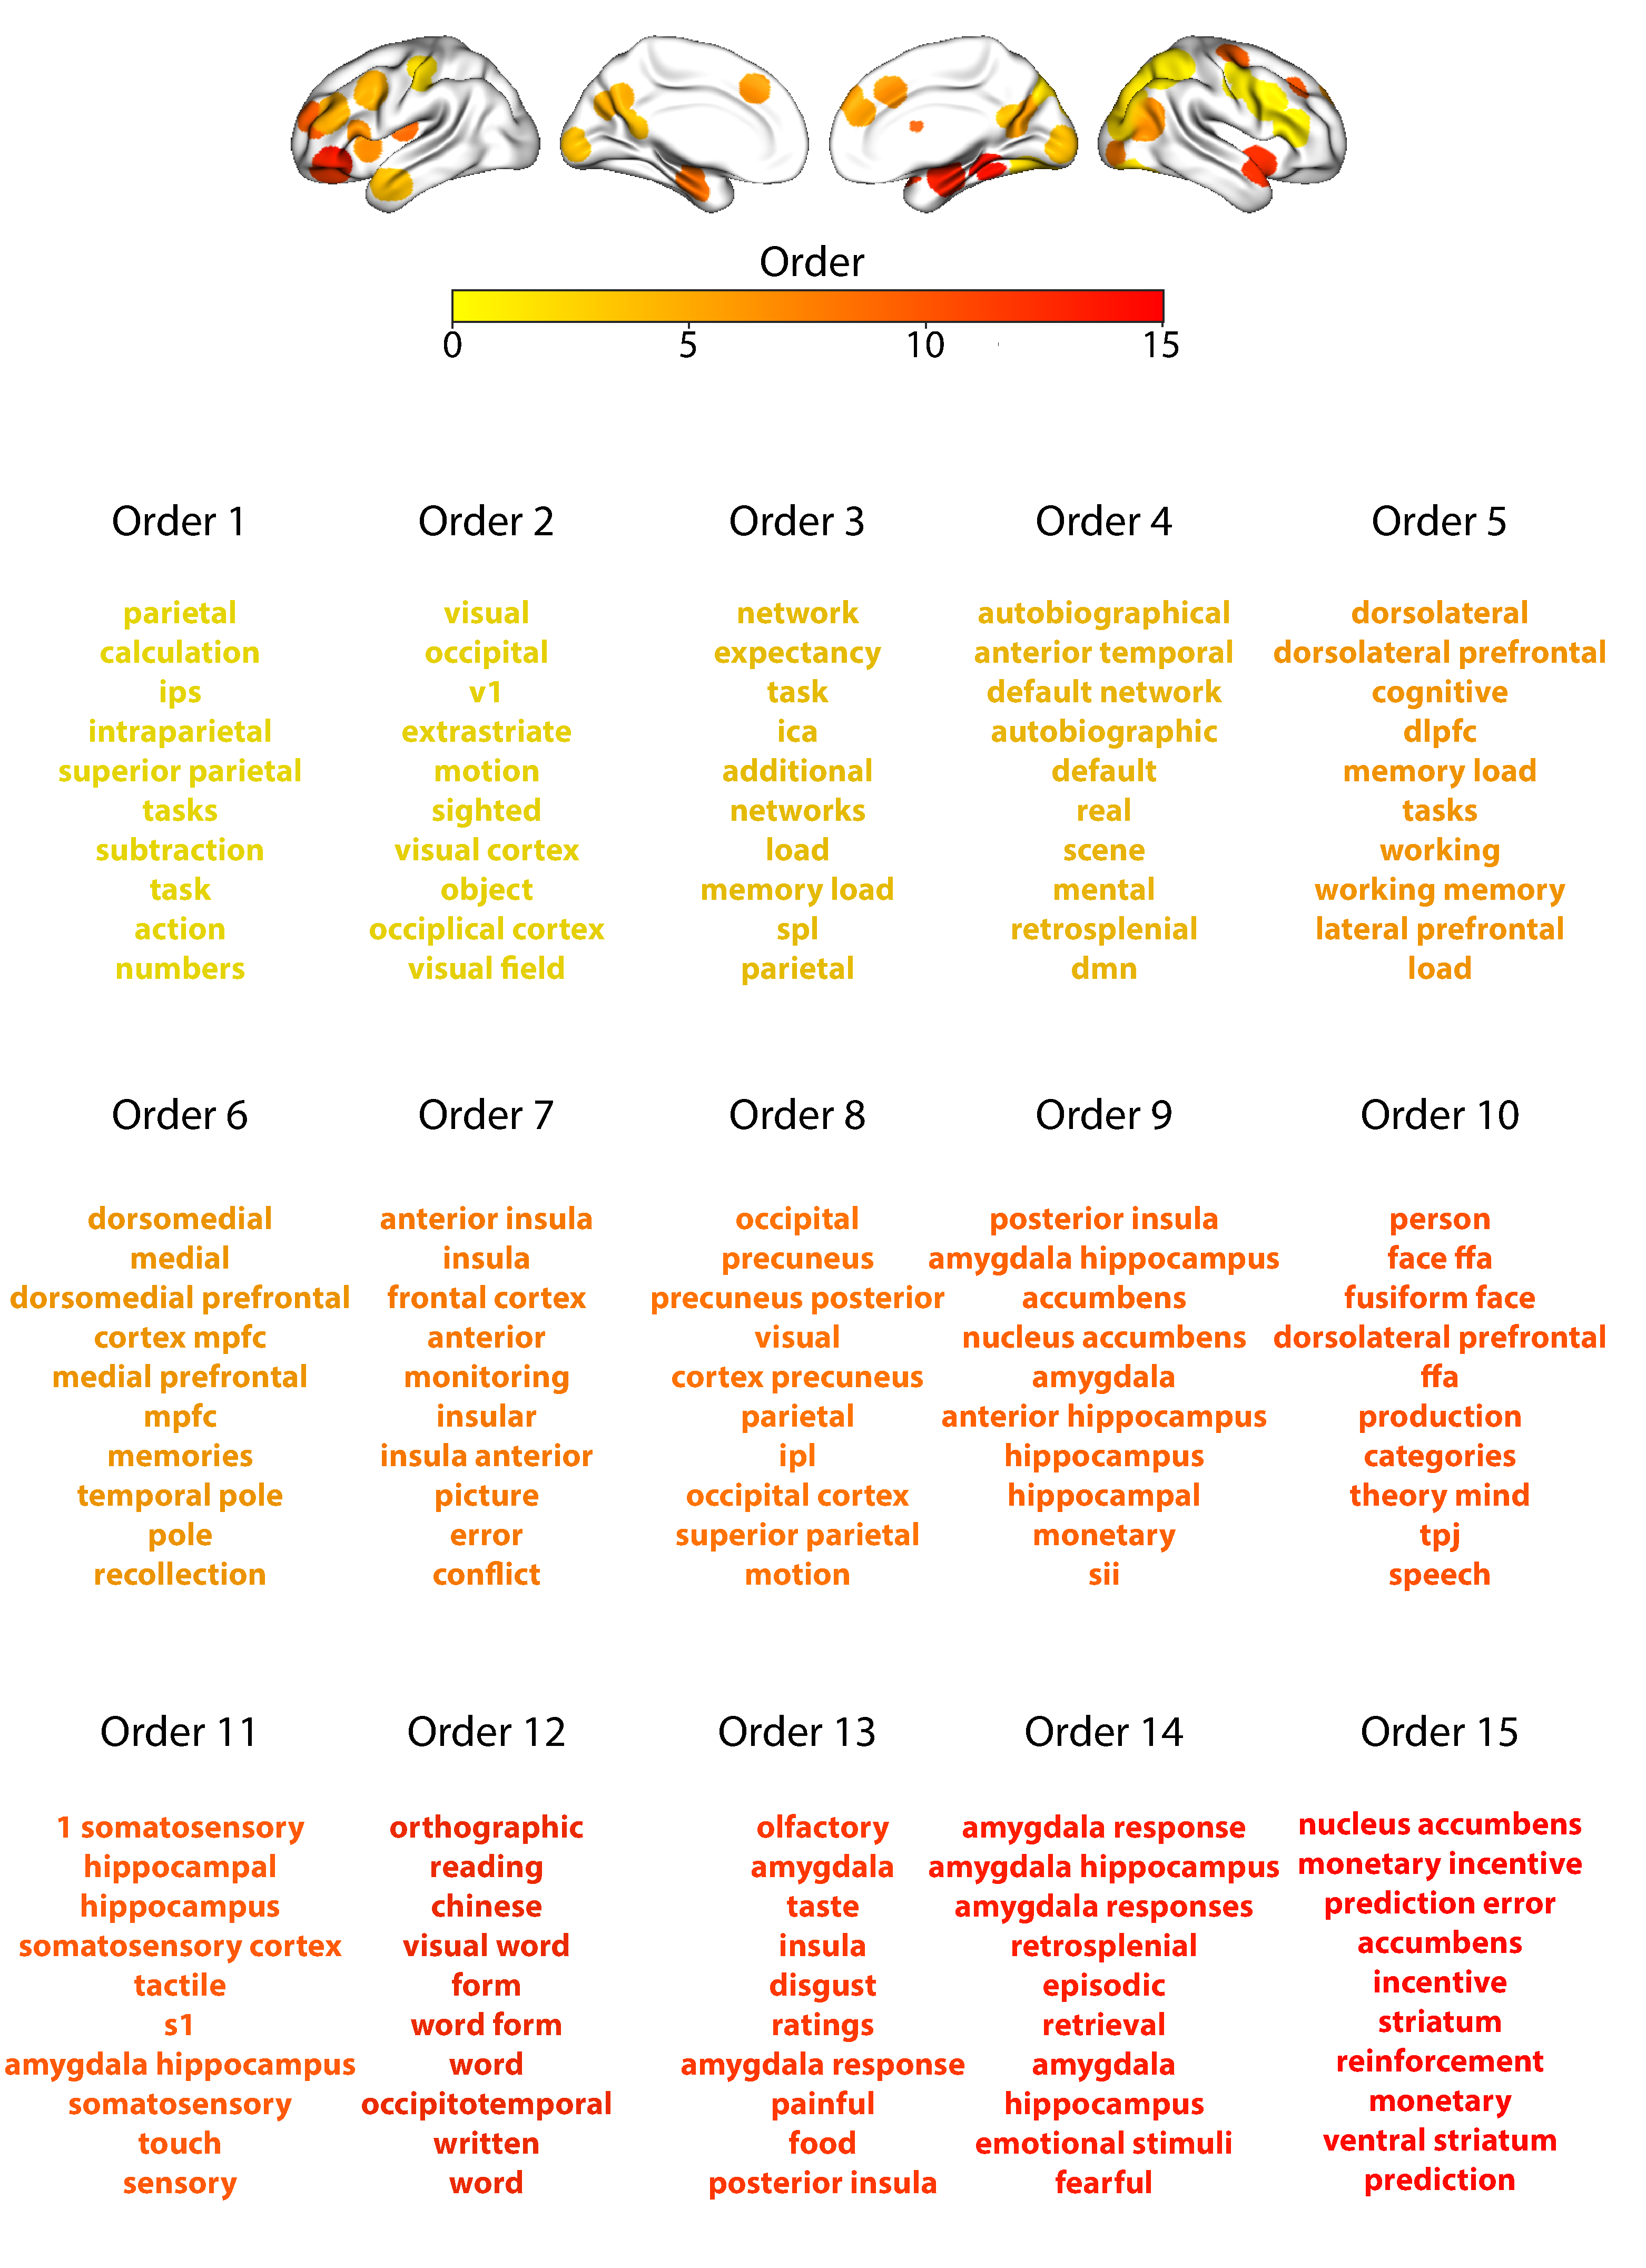
\includegraphics[width=0.75\textwidth]{figs/supp_15_rest}
\caption{\textbf{Top terms associated with the endpoints of the
    strongest correlations for the \textit{rest} experimental
    condition.}  This figure is in the same format as
  Figure~\ref{fig:intact}, but displays results for the
  resting state condition.  (Also see Fig.~\neurosynth,
bottom row, in the main text.)}
\label{fig:rest}
\end{figure}



%\section*{Participant-level figures referenced in the main text}

% Supporting information


\newpage
\renewcommand{\refname}{Supplemental references}
\bibliography{memlab}


\end{document}